%% Beginning of file 'sample631.tex'
%%
%% Modified 2022 May  
%%
%% This is a sample manuscript marked up using the
%% AASTeX v6.31 LaTeX 2e macros.
%%
%% AASTeX is now based on Alexey Vikhlinin's emulateapj.cls 
%% (Copyright 2000-2015).  See the classfile for details.

%% AASTeX requires revtex4-1.cls and other external packages such as
%% latexsym, graphicx, amssymb, longtable, and epsf.  Note that as of 
%% Oct 2020, APS now uses revtex4.2e for its journals but remember that 
%% AASTeX v6+ still uses v4.1. All of these external packages should 
%% already be present in the modern TeX distributions but not always.
%% For example, revtex4.1 seems to be missing in the linux version of
%% TexLive 2020. One should be able to get all packages from www.ctan.org.
%% In particular, revtex v4.1 can be found at 
%% https://www.ctan.org/pkg/revtex4-1.

%% The first piece of markup in an AASTeX v6.x document is the \documentclass
%% command. LaTeX will ignore any data that comes before this command. The 
%% documentclass can take an optional argument to modify the output style.
%% The command below calls the preprint style which will produce a tightly 
%% typeset, one-column, single-spaced document.  It is the default and thus
%% does not need to be explicitly stated.
%%
%% using aastex version 6.3
\documentclass[twocolumn]{aastex631}

\usepackage{verbatim}
\usepackage{amsmath}
\usepackage{multirow}
\usepackage{relsize}


\usepackage{amssymb}
\usepackage{float}
\usepackage{hyperref}

\graphicspath{{figs/}}

\newcommand{\bb}[1]{{\textcolor{blue}{[bb: #1]}}}
\newcommand{\sigs}{\sigma_s}
\newcommand{\dv}[1]{{\color{red}dv: #1}}
\newcommand{\kpo}[1]{{\color{red}kpo: #1}}
\newcommand{\mm}[1]{{\textcolor{purple}{[mm: #1]}}}
%%%%%%%%%%%%%%%%%%%%%%%%%%%%%%%%%%%%%%%%%%%%%%%%%%%%%%%%%%%%%%%%%%%%%%%%%%%%%%%%

%\submitjournal{ApJ}

\shorttitle{Energy Budgets of Galaxy Merger}
\shortauthors{Motka et al.}

%%%%%%%%%%%%%%%%%%%%%%%%%%%%%%%%%%%%%%%%%%%%%%%%%%%%%%%%%%%%%%%%%%%%%%%%%%%%%%%%


%% The default is a single spaced, 10 point font, single spaced article.
%% There are 5 other style options available via an optional argument. They
%% can be invoked like this:
%%
%% \documentclass[arguments]{aastex631}
%% 
%% where the layout options are:
%%
%%  twocolumn   : two text columns, 10 point font, single spaced article.
%%                This is the most compact and represent the final published
%%                derived PDF copy of the accepted manuscript from the publisher
%%  manuscript  : one text column, 12 point font, double spaced article.
%%  preprint    : one text column, 12 point font, single spaced article.  
%%  preprint2   : two text columns, 12 point font, single spaced article.
%%  modern      : a stylish, single text column, 12 point font, article with
%% 		  wider left and right margins. This uses the Daniel
%% 		  Foreman-Mackey and David Hogg design.
%%  RNAAS       : Supresses an abstract. Originally for RNAAS manuscripts 
%%                but now that abstracts are required this is obsolete for
%%                AAS Journals. Authors might need it for other reasons. DO NOT
%%                use \begin{abstract} and \end{abstract} with this style.
%%
%% Note that you can submit to the AAS Journals in any of these 6 styles.
%%
%% There are other optional arguments one can invoke to allow other stylistic
%% actions. The available options are:
%%
%%   astrosymb    : Loads Astrosymb font and define \astrocommands. 
%%   tighten      : Makes baselineskip slightly smaller, only works with 
%%                  the twocolumn substyle.
%%   times        : uses times font instead of the default
%%   linenumbers  : turn on lineno package.
%%   trackchanges : required to see the revision mark up and print its output
%%   longauthor   : Do not use the more compressed footnote style (default) for 
%%                  the author/collaboration/affiliations. Instead print all
%%                  affiliation information after each name. Creates a much 
%%                  longer author list but may be desirable for short 
%%                  author papers.
%% twocolappendix : make 2 column appendix.
%%   anonymous    : Do not show the authors, affiliations and acknowledgments 
%%                  for dual anonymous review.
%%
%% these can be used in any combination, e.g.
%%
%% \documentclass[twocolumn,linenumbers,trackchanges]{aastex631}
%%
%% AASTeX v6.* now includes \hyperref support. While we have built in specific
%% defaults into the classfile you can manually override them with the
%% \hypersetup command. For example,
%%
%% \hypersetup{linkcolor=red,citecolor=green,filecolor=cyan,urlcolor=magenta}
%%
%% will change the color of the internal links to red, the links to the
%% bibliography to green, the file links to cyan, and the external links to
%% magenta. Additional information on \hyperref options can be found here:
%% https://www.tug.org/applications/hyperref/manual.html#x1-40003
%%
%% Note that in v6.3 "bookmarks" has been changed to "true" in hyperref
%% to improve the accessibility of the compiled pdf file.
%%
%% If you want to create your own macros, you can do so
%% using \newcommand. Your macros should appear before
%% the \begin{document} command.
%%
\newcommand{\vdag}{(v)^\dagger}
\newcommand\aastex{AAS\TeX}
\newcommand\latex{La\TeX}

%% Reintroduced the \received and \accepted commands from AASTeX v5.2
%\received{March 1, 2021}
%\revised{April 1, 2021}
%\accepted{\today}

%% Command to document which AAS Journal the manuscript was submitted to.
%% Adds "Submitted to " the argument.
%\submitjournal{PSJ}

%% For manuscript that include authors in collaborations, AASTeX v6.31
%% builds on the \collaboration command to allow greater freedom to 
%% keep the traditional author+affiliation information but only show
%% subsets. The \collaboration command now must appear AFTER the group
%% of authors in the collaboration and it takes TWO arguments. The last
%% is still the collaboration identifier. The text given in this
%% argument is what will be shown in the manuscript. The first argument
%% is the number of author above the \collaboration command to show with
%% the collaboration text. If there are authors that are not part of any
%% collaboration the \nocollaboration command is used. This command takes
%% one argument which is also the number of authors above to show. A
%% dashed line is shown to indicate no collaboration. This example manuscript
%% shows how these commands work to display specific set of authors 
%% on the front page.
%%
%% For manuscript without any need to use \collaboration the 
%% \AuthorCollaborationLimit command from v6.2 can still be used to 
%% show a subset of authors.
%
%\AuthorCollaborationLimit=2
%
%% will only show Schwarz & Muench on the front page of the manuscript
%% (assuming the \collaboration and \nocollaboration commands are
%% commented out).
%%
%% Note that all of the author will be shown in the published article.
%% This feature is meant to be used prior to acceptance to make the
%% front end of a long author article more manageable. Please do not use
%% this functionality for manuscripts with less than 20 authors. Conversely,
%% please do use this when the number of authors exceeds 40.
%%
%% Use \allauthors at the manuscript end to show the full author list.
%% This command should only be used with \AuthorCollaborationLimit is used.

%% The following command can be used to set the latex table counters.  It
%% is needed in this document because it uses a mix of latex tabular and
%% AASTeX deluxetables.  In general it should not be needed.
%\setcounter{table}{1}

%%%%%%%%%%%%%%%%%%%%%%%%%%%%%%%%%%%%%%%%%%%%%%%%%%%%%%%%%%%%%%%%%%%%%%%%%%%%%%%%
%%
%% The following section outlines numerous optional output that
%% can be displayed in the front matter or as running meta-data.
%%
%% If you wish, you may supply running head information, although
%% this information may be modified by the editorial offices.
%\shorttitle{AASTeX v6.3.1 Sample article}
%\shortauthors{Schwarz et al.}
%%
%% You can add a light gray and diagonal water-mark to the first page 
%% with this command:
%% \watermark{text}
%% where "text", e.g. DRAFT, is the text to appear.  If the text is 
%% long you can control the water-mark size with:
%% \setwatermarkfontsize{dimension}
%% where dimension is any recognized LaTeX dimension, e.g. pt, in, etc.
%%
%%%%%%%%%%%%%%%%%%%%%%%%%%%%%%%%%%%%%%%%%%%%%%%%%%%%%%%%%%%%%%%%%%%%%%%%%%%%%%%%
%\graphicspath{{./}{figures/}}
%% This is the end of the preamble.  Indicate the beginning of the
%% manuscript itself with \begin{document}.

\begin{document}

\title{Transformations of Internal Energy Budgets during the Formation of Major MW-M31 Merger Remnant Samyog}

%% LaTeX will automatically break titles if they run longer than
%% one line. However, you may use \\ to force a line break if
%% you desire. In v6.31 you can include a footnote in the title.

%% A significant change from earlier AASTEX versions is in the structure for 
%% calling author and affiliations. The change was necessary to implement 
%% auto-indexing of affiliations which prior was a manual process that could 
%% easily be tedious in large author manuscripts.
%%
%% The \author command is the same as before except it now takes an optional
%% argument which is the 16 digit ORCID. The syntax is:
%% \author[xxxx-xxxx-xxxx-xxxx]{Author Name}
%%
%% This will hyperlink the author name to the author's ORCID page. Note that
%% during compilation, LaTeX will do some limited checking of the format of
%% the ID to make sure it is valid. If the "orcid-ID.png" image file is 
%% present or in the LaTeX pathway, the OrcID icon will appear next to
%% the authors name.
%%
%% Use \affiliation for affiliation information. The old \affil is now aliased
%% to \affiliation. AASTeX v6.31 will automatically index these in the header.
%% When a duplicate is found its index will be the same as its previous entry.
%%
%% Note that \altaffilmark and \altaffiltext have been removed and thus 
%% can not be used to document secondary affiliations. If they are used latex
%% will issue a specific error message and quit. Please use multiple 
%% \affiliation calls for to document more than one affiliation.
%%
%% The new \altaffiliation can be used to indicate some secondary information
%% such as fellowships. This command produces a non-numeric footnote that is
%% set away from the numeric \affiliation footnotes.  NOTE that if an
%% \altaffiliation command is used it must come BEFORE the \affiliation call,
%% right after the \author command, in order to place the footnotes in
%% the proper location.
%%
%% Use \email to set provide email addresses. Each \email will appear on its
%% own line so you can put multiple email address in one \email call. A new
%% \correspondingauthor command is available in V6.31 to identify the
%% corresponding author of the manuscript. It is the author's responsibility
%% to make sure this name is also in the author list.
%%
%% While authors can be grouped inside the same \author and \affiliation
%% commands it is better to have a single author for each. This allows for
%% one to exploit all the new benefits and should make book-keeping easier.
%%
%% If done correctly the peer review system will be able to
%% automatically put the author and affiliation information from the manuscript
%% and save the corresponding author the trouble of entering it by hand.

%\correspondingauthor{August Muench}
%\email{greg.schwarz@aas.org, gus.muench@aas.org}
\correspondingauthor{Jay Motka}
\email{jaymotka@arizona.edu}

\author[0000-0001-7379-2625]{Jay Motka} 
\affiliation{Department of Astronomy and Steward Observatory, University of Arizona, Tucson, AZ 85721, USA}
\affiliation{Department of Physics, University of Arizona, Tucson, AZ 85721, USA}
\date{May 5, 2023}

%% Note that the \and command from previous versions of AASTeX is now
%% depreciated in this version as it is no longer necessary. AASTeX 
%% automatically takes care of all commas and "and"s between authors names.

%% AASTeX 6.31 has the new \collaboration and \nocollaboration commands to
%% provide the collaboration status of a group of authors. These commands 
%% can be used either before or after the list of corresponding authors. The
%% argument for \collaboration is the collaboration identifier. Authors are
%% encouraged to surround collaboration identifiers with ()s. The 
%% \nocollaboration command takes no argument and exists to indicate that
%% the nearby authors are not part of surrounding collaborations.

%% Mark off the abstract in the ``abstract'' environment. 
\begin{abstract}
    We investigate the evolution of internal energy budgets of the dark matter halos in the initial three-galaxy system of Milky Way (MW), Andromeda galaxy (M31), and Triangulam galaxy (M33) during the formation of major MW-M31 merger remnant, Samyog. The exchange of energies within the system governs the structural evolution of the halos within the system. By looking at the evolution of the internal energy budgets and virial ratios of the halos, we investigate whether the halo of the major merger remnant Samyog is dominantly supported by velocity dispersion or rotation. We also investigate whether the M33 halo gains or loses energy during the formation of Samyog and how it changes its internal structure. Through this investigation, we get a better understanding of the evolution of halos of major merger remnant as well as the smaller satellite in a complex system of galaxies as the merger takes place. We found the final virial ratio of Samyog to be $\lambda_{vir} = 0.760$. This indicates that the major merger remnants like Samyog are dominantly dispersion supported in such complex systems after the mergers take place. We also found that M33 gains an abundance of energy such that its total energy becomes positive and its virial ratio becomes very small after the merger. This indicates that many dark matter particles are tidally stripped from the halos of small satellite galaxies like M33 in such complex systems as the mergers take place.  
\end{abstract}

\keywords{Local Group; Galaxy Merger; Merger Remnant; Major Merger; Dark Matter Halo; Virial Equilibrium}

\section{Introduction}
\label{sec:intro}
Milky Way (MW) along with its largest neighbour the Andromeda galaxy (M31) and a collection of the satellite galaxies that orbit them make up a group of galaxies called the Local Group. The largest of these satellite galaxies is the Triangulum galaxy (M33). According to \cite{simulation}, the MW and M31 will merge at $t = 5.86^{+1.61}_{-0.13}$ Gyr from now. A galaxy merger happens when a system of interacting galaxies collide with each other. This system is defined to be merged once their nuclei have coalesced and there is only one central luminosity peak that remains. This merged system is known as merger remnant. When the interacting galaxy pairs have the luminosity ratio of $L_2/L_1 > 0.33$, the galaxy merger is known as major merger and the merger remnant is known as major merger remnant \citep{major_merger_def}. The MW-M31 merger is a major merger, and the major merger remnant of MW-M31 system is often called Milkomeda or Milkdromeda in popular sources. On the account of preserving the integrity of the originality in naming cosmological objects in the astronomy community, for the purposes of this paper, we name the major merger remnant of MW-M31 system as the Sanskrit word ``Samyog'', translating to English as ``a merger'' or ``an union''. Using the N-body simulation described in \cite{simulation}, we propose to study the evolution of internal energy budgets in the system made of MW, M31, and M33 as the merger between MW and M31 takes place. 

As defined in \cite{galaxy_def}, ``A galaxy is a gravitationally bound collection of stars whose properties cannot be explained by a combination of baryons and Newton’s laws of gravity''. A Galaxy evolves over time through many ways, including the changes in its structure, gas mass, stellar mass, or color. However, a galaxy merger can speed this process of galaxy evolution many folds. The distribution of internal and orbital energy of the system can tell us a lot about the structure of individual galaxies as well as system as a whole. The spherical distribution of dark matter (DM) that surrounds the baryonic disk or spheroid of a galaxy is known as the dark matter halo, simply referred to as halo from now on. As the halos are the most massive components of galaxies, the exchange of energies is an excellent tracer of the evolution of the structures of halos. Thus, it is important to understand the evolution of various energy budgets of a DM halos in a system during a merger. 

We currently have an understanding of the energy evolution of the halos in a system of two galaxies as they merge \citep[e.g.][]{same_mass_merger_1, same_mass_merger_2}. The virial ratio of a galaxy is defined as, 
\begin{align}
    \lambda_{vir} = - \frac{P}{2K},
    \label{eq:virial_ratio}
\end{align}
where $P$ is the total internal potential energy and $K$ is the total kinetic energy \citep{same_mass_merger_1}. When the virial ratio equals to 1, the galaxy is in virial equilibrium and is purely supported by velocity dispersion. Fig. \ref{fig:virial}, taken from \cite{same_mass_merger_1}, shows the merger remnant of two equal mass galaxies that is dominantly supported by velocity dispersion.

\begin{figure}[htbp]
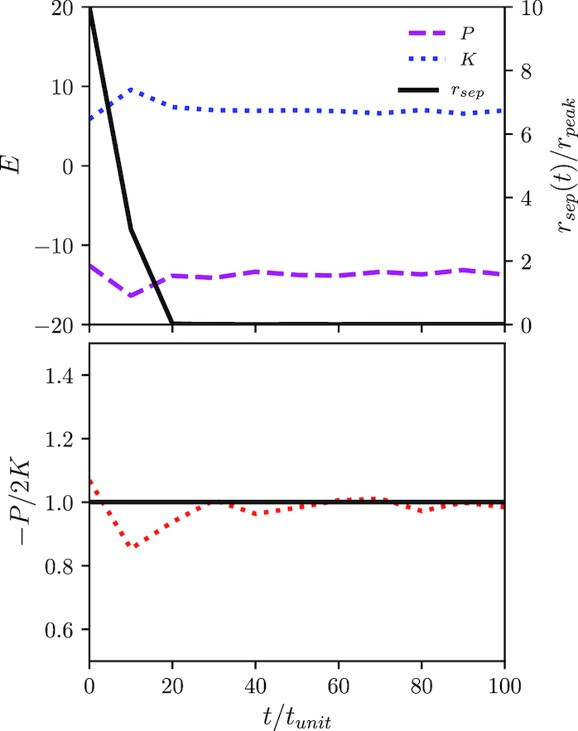
\includegraphics[width=.5\textwidth]{two_galaxy_merger.jpg}
\caption{Energy evolution of the system of two halos of the same mass, merging together, as shown in \cite{same_mass_merger_1}. The progenitor galaxies possessed the Einasto density profiles. As can be seen in the bottom panel, after the merger, virial ratio (dotted red line) of the merger halo is nearly equal to 1.\label{fig:virial}}
\end{figure}

For a system of two galaxies, the total energy of the two galaxies remains conserved as they merge into a single remnant as is obvious in the case of the simulation of two-galaxy system \citep{same_mass_merger_1}. However, we do not yet have a sound understanding of how the energy evolves in a more complex system containing more than two galaxies, which is the case in most galaxy mergers. As the given simulation contains a three-galaxy system, it is possible that the total energy of the MW and M31 may not remain conserved as there may be energy loss or gain from their interaction with M33. Understanding this interaction helps us understand the open problem of understanding galaxy mergers in systems with multiple galaxies. Furthermore, It is known that known halo shapes are mostly supported dominantly by anisotropic velocity dispersion as they rotate very slowly \citep{spin_param_explain}. However, do the halos of major merger remnants like Samyog also follow this theory? It is also unknown how the structure of small satellite galaxies change as the major merger occurs in the complex galaxy systems. Finding answers to these open questions is essential to further understand the galaxy evolution through mergers occurring within complex systems like our local group. 

\section{This Project}
\label{sec:proj}
In this paper, we propose to investigate whether the halo of major merger remnant Samyog is supported by rotation or velocity dispersion by looking at its virial ratio. We also look at the internal energy budgets of M33 as it evolves over time. For these purposes, we want to understand the distribution of internal energies of the three halos before the merger and compare them to the final distribution of internal energies of the halos of Samyog and M33. 

This project addresses both the open questions mentioned in Section \ref{sec:intro}. We find out whether the halo of Samyog is dominantly dispersion supported or dominantly rotation supported. We also investigate whether the halo of M33 gains energy or looses energy and how that changes its internal structure in terms of it being more dispersion depended or more rotation depended as the merger takes place.

The information of whether the galaxy halo is dispersion supported or rotation supported corresponds to the internal structure, density profile, and shape of the galaxy \citep{same_mass_merger_1, same_mass_merger_2}. Thus, answering the proposed questions is something very important in understanding galaxy evolution through a major merger. This project addresses these questions by looking at the different internal energy budgets of all the separate halos at a given time. Using those internal energy budgets, we find the virial ratios for all the halos, which are the direct indicators of whether the halos are dominantly supported by dispersion or not.   


\section{Methodology}
\label{sec:method}

Based on the current observational data, the future interactions between MW and M31 galaxies have been studied broadly. One such study was carried out using a combination of collisionless N-body simulations and semi-analytic orbit integrations for the three-galaxy system of MW, M31, and M33 in \cite{simulation}. Here, the N-body simulation means a dynamical simulation of system of many particles governed by the gravitational force. In this paper, we utilize this N-body simulation to investigate our questions. 

\begin{figure}[htbp]
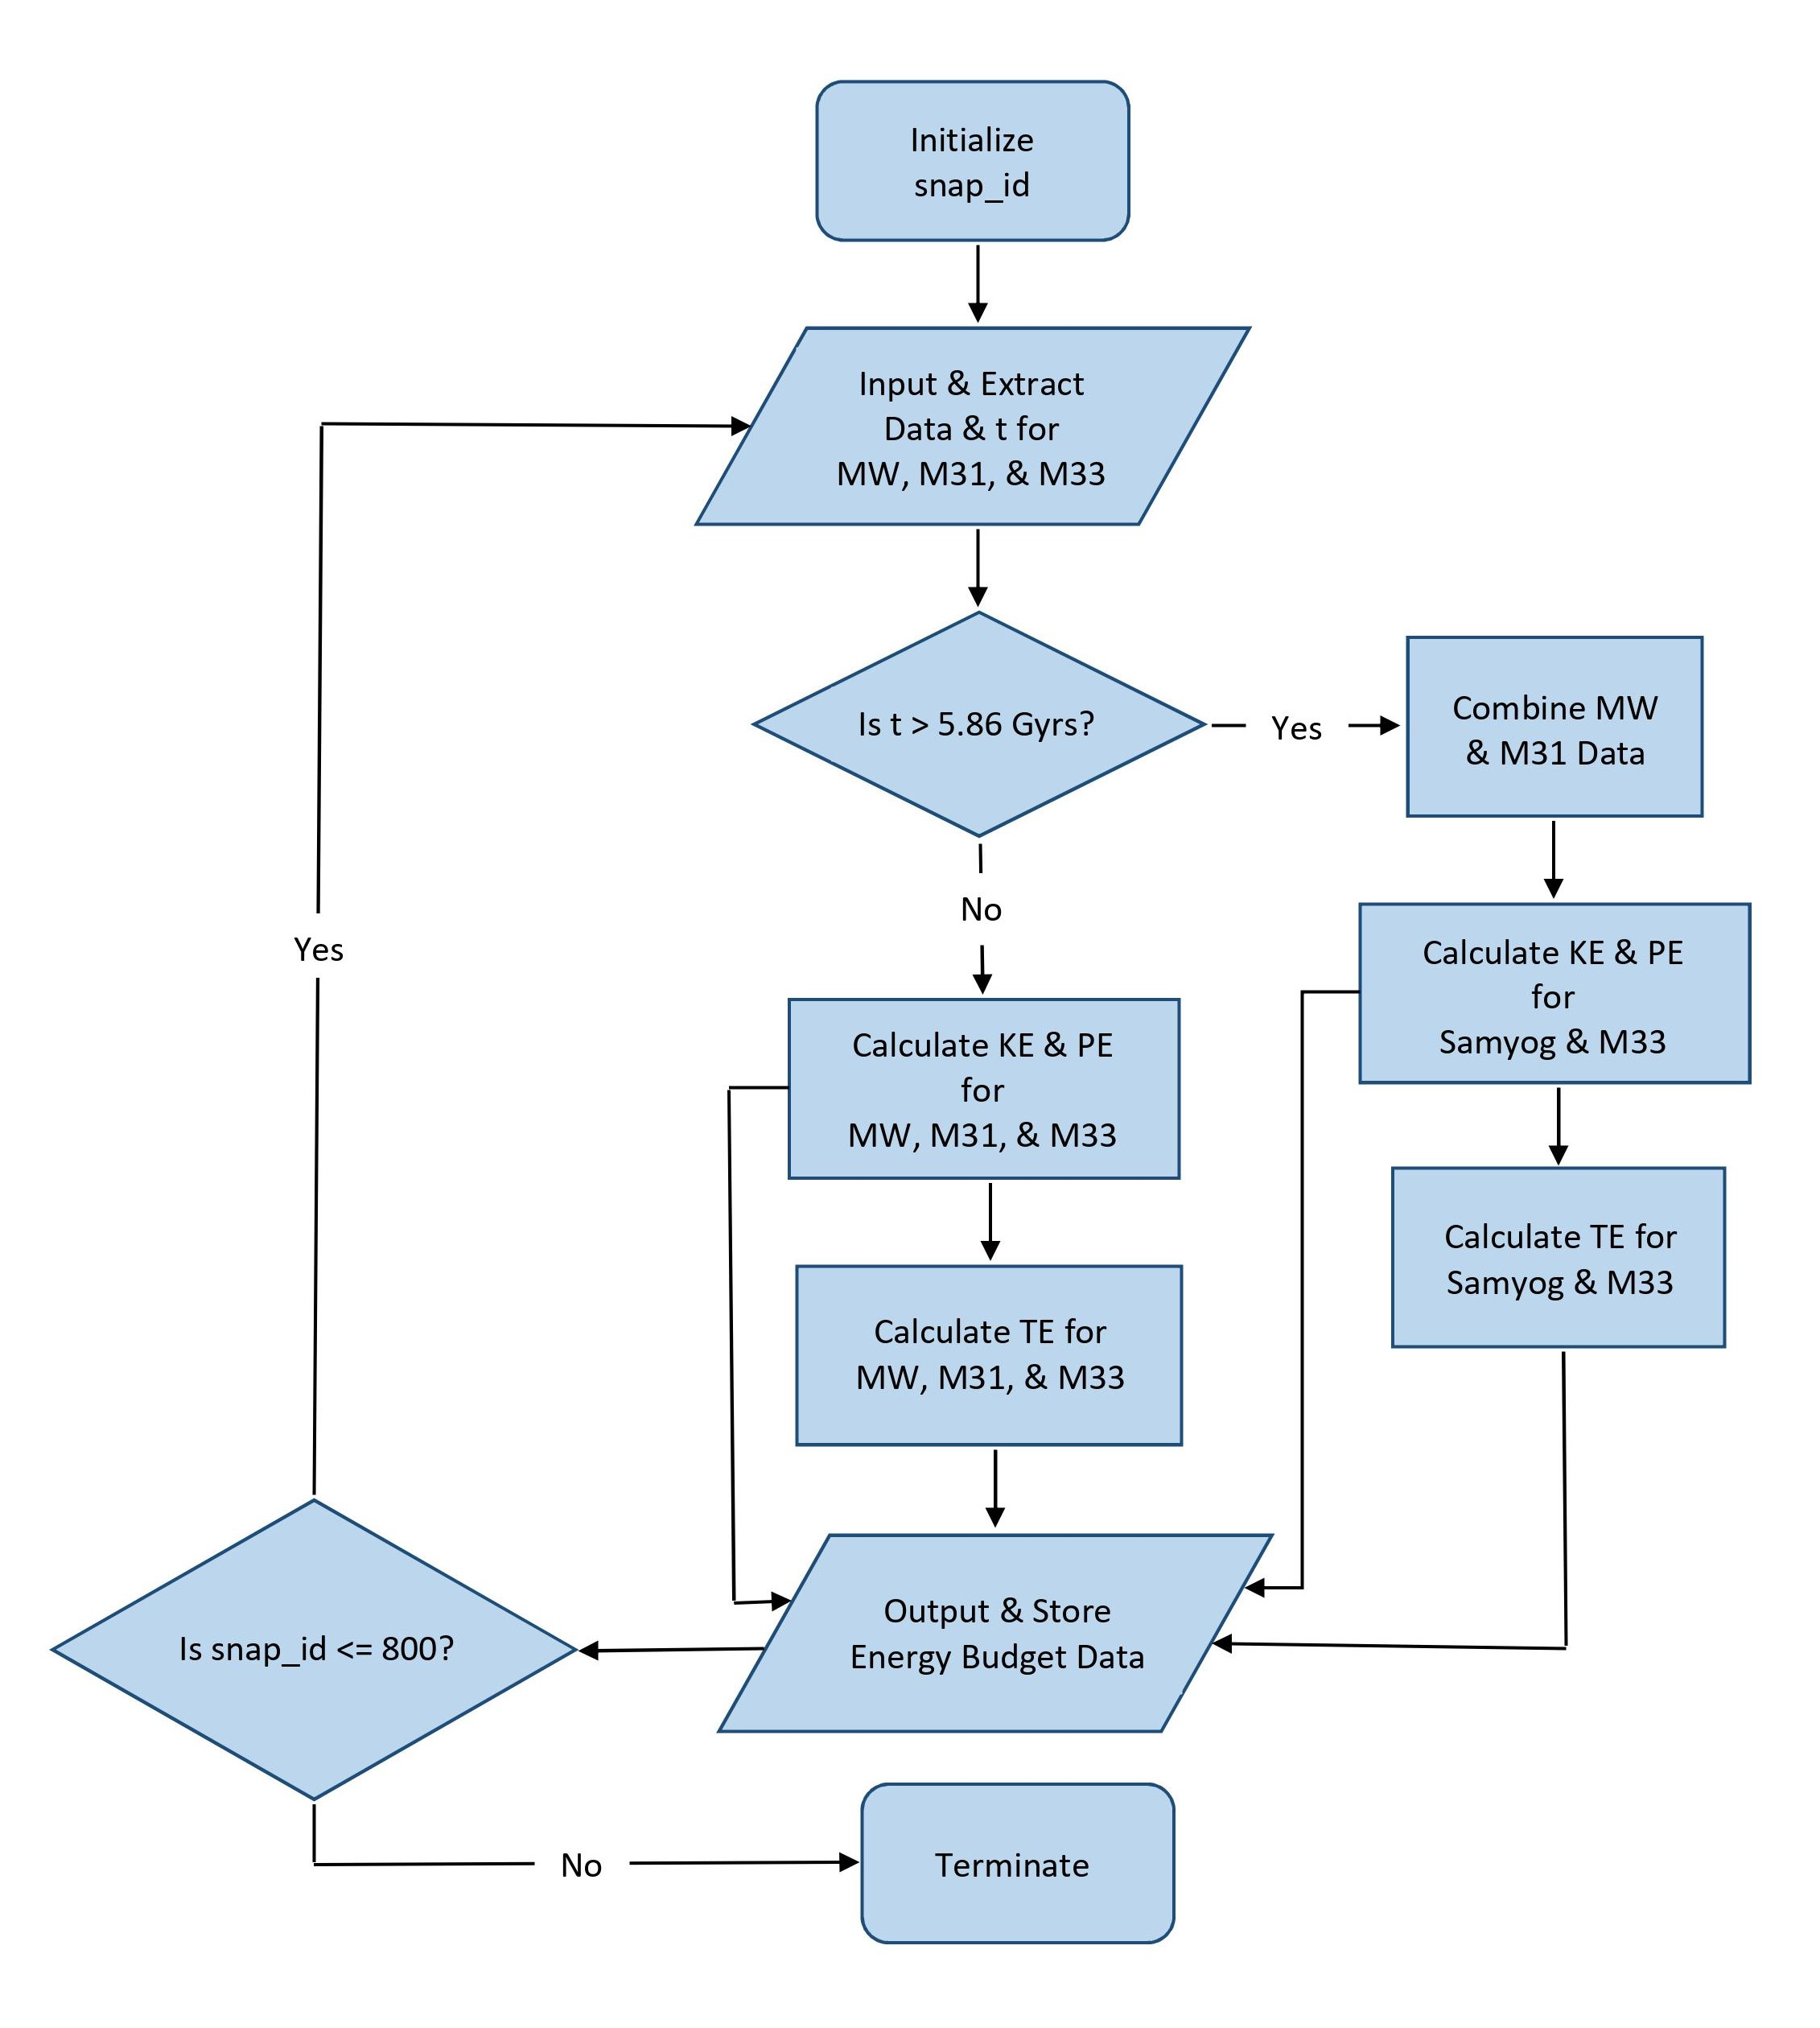
\includegraphics[width=.5\textwidth]{flowchart.jpg}
\caption{Flowchart showing the process of calculating internal energy budgets of different halos evolving with time. Note that the MW and M31 data is combined to calculate the internal energy budgets of the halo of Samyog after time $t > 5.86$ Gyr \citep{simulation}.
\label{fig:flowchart}}
\end{figure}

To answer these questions, we calculate the internal energies of the various halos according to the flowchart shown in Fig. \ref{fig:flowchart}. We first calculate the internal energies of MW, M31, and M33 halos at given times before the merger occurs, i.e. at $t < 5.86$ Gyr \citep[see][]{simulation}. After the merger, we calculate the internal energies of Samyog and M33 halos at given times. We then calculate the virial ratios of Samyog's halo, at given times to see how it evolves after its formation. We compare the virial ratios of MW and M33 halos at $t=0$ Gyr with the virial ratio evolution of Samyog's halo to understand the halo structure of a galaxy major merger compared to its progenitors. Finally, we look at the evolution of M33 halo's virial ratio throughout the merger process to understand merger's impact on the satellite galaxy. Comparing the internal energies of M33 before and after the merger allows us to understand how it evolves as the merger takes place.

We investigate the total internal energies of the halos as the merger occurs. This is done by using the equation for internal energy of the particular galaxy,
\begin{align}
    E_{int,g} = K_{int,g} + P_{int,g},
    \label{eq:internal_energy}
\end{align}
where $K_{int,g}$ is the internal kinetic energy of the halo and $P_{int,g}$ is the internal potential energy of the halo. These can be found using,
\begin{align}
    K_{int,g} &=\frac{1}{2}\Sigma_{i=1}^N m_i v_i^2, \nonumber \\ 
    P_{int,g} &= - \Sigma_{i\neq j}^{N} \frac{G m_i m_j}{r_{ij}},
    \label{eq:kinetic_and_potential_energy}
\end{align}
where $N$ is the total number of particles in the given galaxy, $m_i$s are the masses of individual dark matter particles, $v_i$s are their speeds, and $r_{i,j}$s are the separations between the two given dark matter particles.

\begin{figure}[htbp]
    \begin{subfigure}
    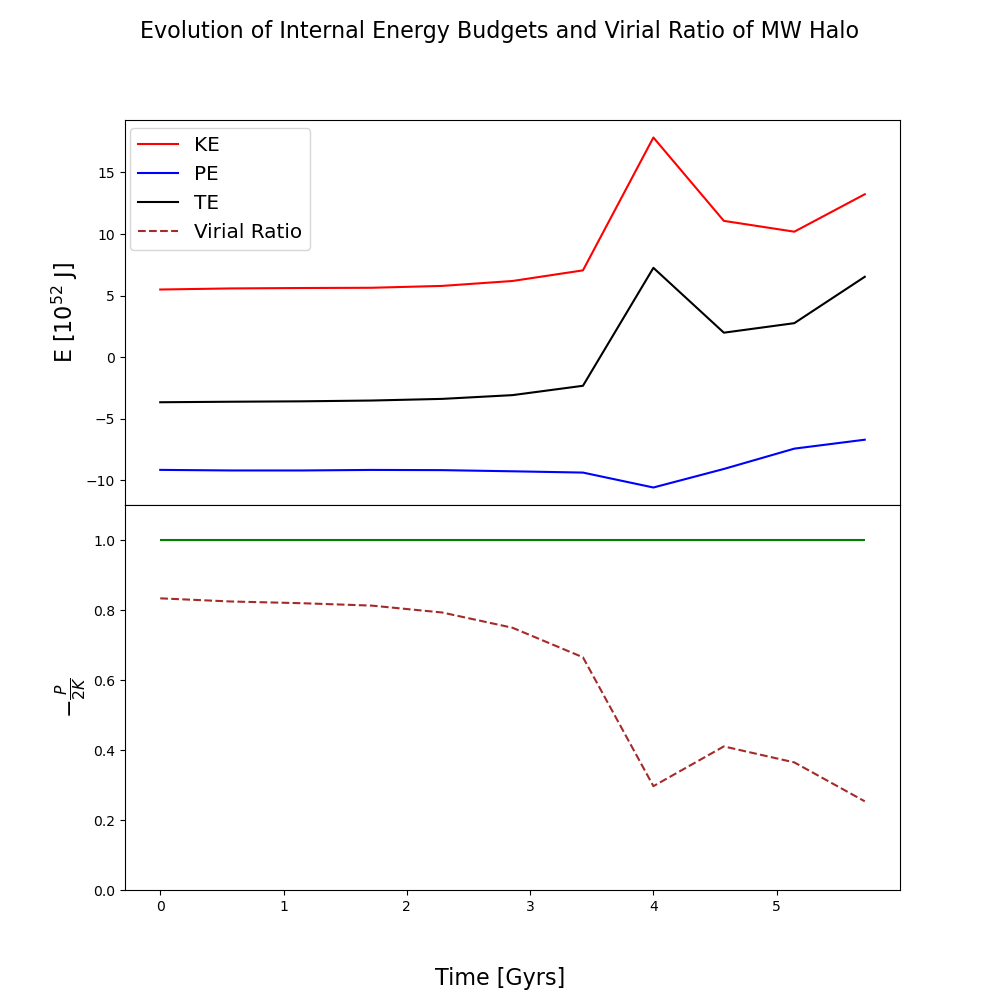
\includegraphics[width=.5\textwidth]{MW_energies_virial_ratios.png}
    \end{subfigure} \\
    \begin{subfigure}
    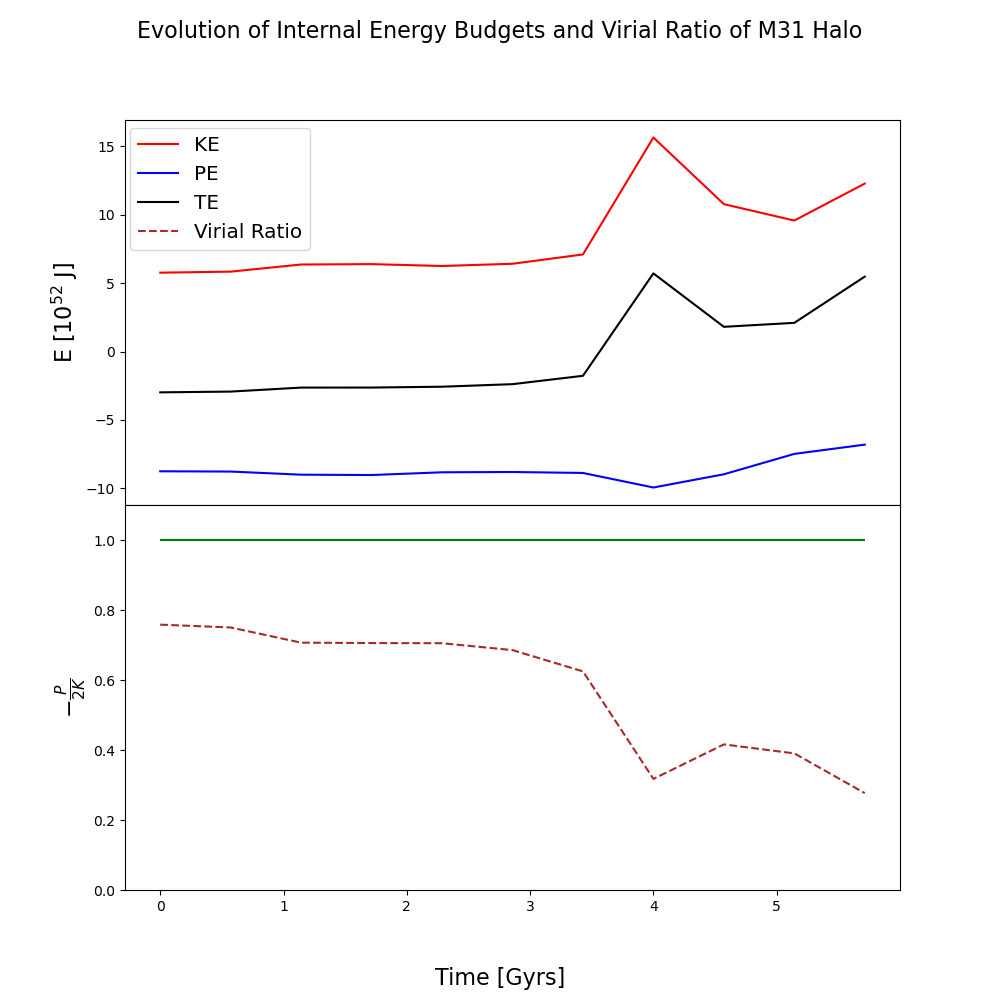
\includegraphics[width=.5\textwidth]{M31_energies_virial_ratios.png}
    \end{subfigure}
\caption{Internal energy and virial ratio evolution of MW (upper) and M31 (lower) before $t=5.86$ Gyrs. The x-axis of both plots show time in Gyrs. The upper part of both plots show the evolution of kinetic energies (red lines), potential energies (blue lines), and total energies (black lines) in $10^{52}$ J. The lower parts of both plots show the evolution of the virial ratios (dashed brown lines) and the references of $\lambda_{vir}=1$ (green lines). As can be seen, both MW and M31 have initial virial ratios that indicate their high dispersion dependence before the merger. 
\label{fig:progen_plot}}
\end{figure}

\begin{figure}[htbp]
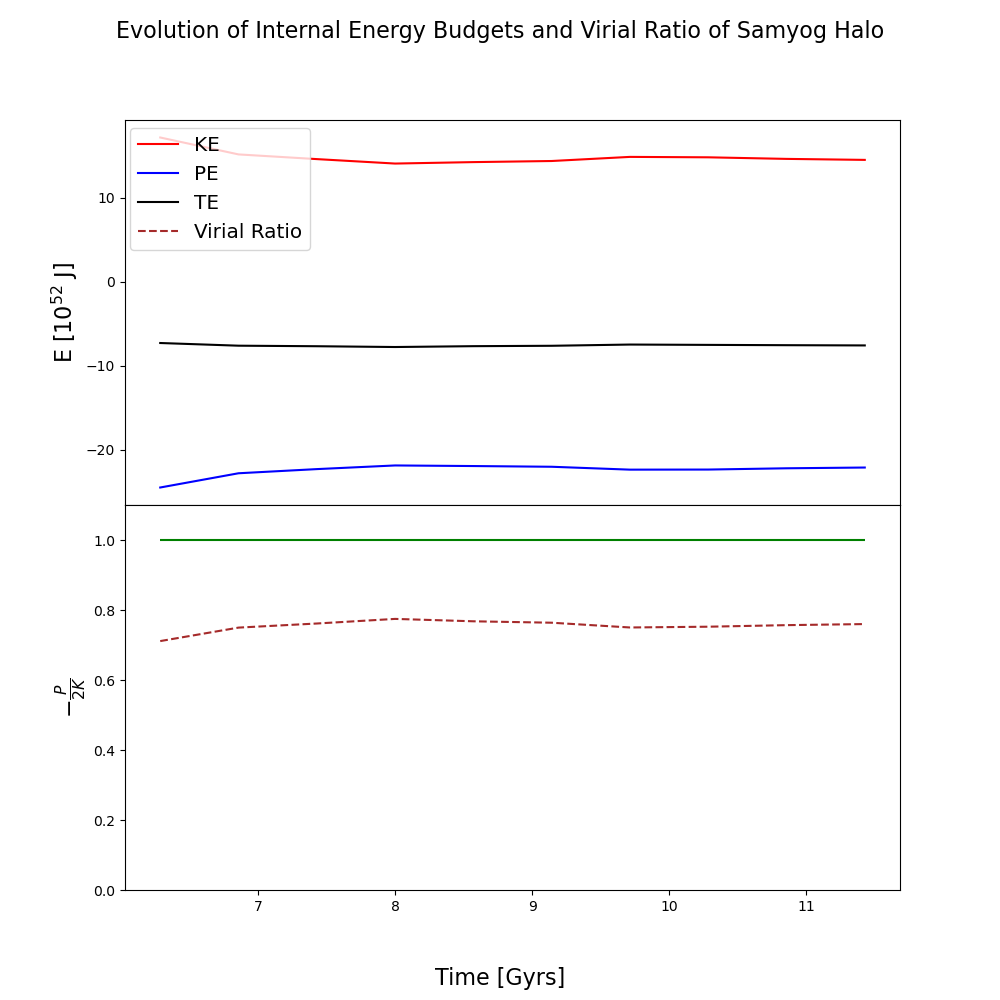
\includegraphics[width=.5\textwidth]{Samyog_energies_virial_ratios.png}
\caption{Internal energy and virial ratio evolution of Samyog after $t=5.86$ Gyr. The x-axis of the plot show time in Gyrs. The upper part of the plot shows the evolution of kinetic energy (red line), potential energy (blue line), and total energy (black line) in $10^{52}$ J. The lower part of the plot shows the evolution of the virial ratio (dashed brown line) and the reference of $\lambda_{vir}=1$ (green line). As can be seen, Samyog has the final virial ratio that indicates its high dispersion dependence after the merger.
\label{fig:Samyog_plot}}
\end{figure}

\begin{figure}[htbp]
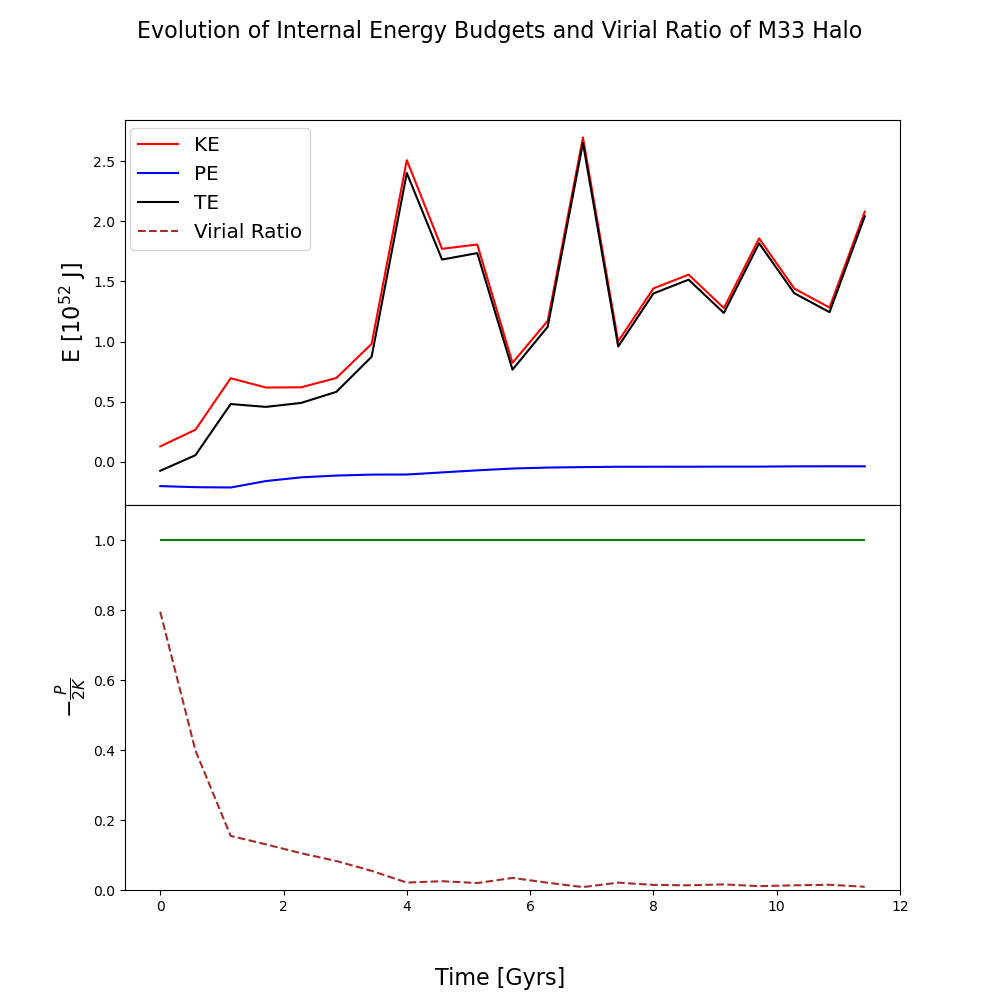
\includegraphics[width=.5\textwidth]{M33_energies_virial_ratios.png}
\caption{Internal energy and virial ratio evolution of M33. The x-axis of the plot shows time in Gyrs. The upper part of the plot shows the evolution of kinetic energy (red line), potential energy (blue line), and total energy (black line) in $10^{52}$ J. The lower part of the plot shows the evolution of the virial ratio (dashed brown line) and the reference of $\lambda_{vir}=1$ (green line). As can be seen, M33 has the initial virial ratio that indicates its high dispersion dependence before the merger and the final virial ratio that indicates its high rotation dependence after the merger.
\label{fig:M33_plot}}
\end{figure}

We plot four figures as part of our results. The first two figures contain the plots of virial ratios and internal energies, similar to Fig. \ref{fig:virial}, of MW and M31 before the merger. The third figure contains the similar plot of Samyog after the merger. The final figure contains the similar plot of M33 over the entirety of the simulation time. Looking at the internal energy budgets evolution as well as the evolution of the virial ratios as the merger occurs would help us understand where the energy goes as well as how the internal structures of the galaxies change as the merger occurs.

We hypothesize that Samyog will be found to be nearer to the virial equilibrium compared to the initial conditions of MW and M31. It is understandable that the major merger remnant, Samyog, will be `hotter' than either MW or M31 at $t=0$ Gyr. This means that the motion of dark matter particles within the halo is more random, giving us a virial ratio for the halo of Samyog to be nearer to 1. Thus, Samyog would be dominantly supported by velocity dispersion. We also hypothesize that M33 will gain internal energy and become more random as it is loosing its orbital energy due to dynamical friction. 

\section{Results}
\label{sec:res}

Using the method shown in Section \ref{sec:method}, we produced four different plots of the evolution of internal energies and virial ratios of the various halos as the merger occurs. The plots of the evolution of internal energies and virial ratios for MW and M31 are given in Fig. \ref{fig:progen_plot}. As can be seen in Fig. \ref{fig:progen_plot}, at $t=0$ Gyr, the virial ratio of MW halo is $\lambda_{vir} = 0.833$ and the virial ratio of M31 halo is $\lambda_{vir} = 0.758$. These initial virial ratios indicate that both MW and M31 are dominantly supported by dispersion before the merger.

The plot of the evolution of internal energies and virial ratio of Samyog are given in Fig. \ref{fig:Samyog_plot}. As can be seen in Fig. \ref{fig:Samyog_plot}, at $t=11.429$ Gyrs, the virial ratio of Samyog halo is $\lambda_{vir} = 0.760$. This final virial ratio of Samyog indicates that Samyog is dominantly supported by dispersion after the merger. Compared to MW before the merger, Samyog has a lower virial ratio, indicating that Samyog is less dispersion dependent than MW. Compared to M31 before the merger, Samyog has very similar but slightly higher virial ratio, indicating that Samyog is slightly more dispersion dependent than M31.

The plot of the evolution of internal energies and virial ratio of M33 are given in Fig. \ref{fig:M33_plot}. As can be seen in Fig. \ref{fig:M33_plot}, the virial ratios of M33 are $\lambda_{vir} = 0.795$ at $t=0$ Gyr and $\lambda_{vir} = 0.009$ at $t=11.429$ Gyrs. This virial ratios indicate that M33 is dominantly supported by dispersion before the merger and appears to be supported by rotation after the merger. We also see that the M33 is gaining significant amount of energy as the merger takes place. 

\section{Discussion}
\label{sec:disc}
As stated in Section \ref{sec:res}, Samyog has the final virial ratio of $\lambda_{vir} = 0.760$. Thus, Samyog is dominantly supported by velocity dispersion. This is similar to what we hypothesized. We also found that it is less dispersion dependent compared to MW before the merger and slightly more dispersion dependent compared to M31 before the merger. This means that two dispersion dependent galaxy halos merge to create a merger halo that is dominantly supported by velocity dispersion. However, it is not necessarily true that it will be more dispersion dependent compared to both of its progenitors. 

These calculations of virial ratios are done by calculating total internal energies of various halos instead of average internal energies. Thus, while these virial ratios gives us an understanding of the big picture, more accurate results would be obtained if we calculate the average internal energies.

As stated in Section \ref{sec:res}, M33 has virial ratios of $\lambda_{vir} = 0.795$ at $t=0$ Gyr and $\lambda_{vir} = 0.009$ at $t=11.429$ Gyrs, indicating that M33 is dominantly supported by dispersion before the merger and appears to be supported by rotation after the merger. We see that the total energy of the M33 is positive after the merger, indicating that the halo of M33 is gravitationally unbound. This indicates that there are many dark matter particles that were stripped from M33. We can see this in Fig. \ref{fig:halo_M33}, where we see the tidally stripped dark matter particles at $t=11.4$ Gyrs. In Fig. \ref{fig:M33_plot}, we also see that the M33 is gaining significant amount of energy as the merger takes place. This is according to what we hypothesized. This means that, in a three-galaxy complex system like MW-M31-M33, when a major merger takes place, the satellite galaxy usually gains energy, resulting in tidal stripping and changing of its internal structure significantly. 

The bipolar velocity distribution seen in the plots of M33 halo at $t=11.4$ Gyrs in Fig. \ref{fig:halo_M33}, is the effect of the stripped dark matter particles, which gives us the found rotational dependence of all the dark matter particles within the initial halo of the M33, indicated by the low virial ratio. This explains the final virial ratio of M33 halo being very low. For more accurate result, we need to define the Jacobi radius of M33 after the merger and calculate internal energies only using particles within that radius. 

\begin{figure*}[htbp]
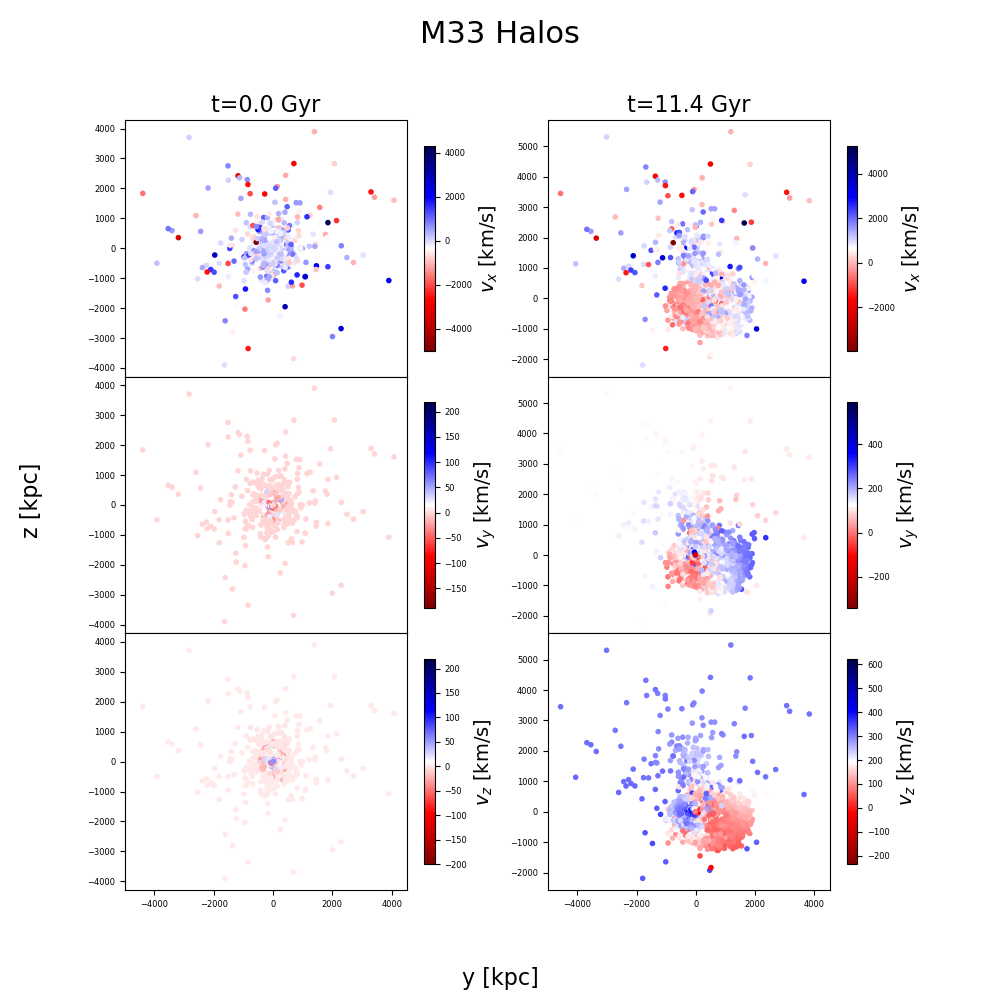
\includegraphics[width=\textwidth]{M33.png}
\caption{Dark matter halos of the M33 galaxy. The left three plots and the right three plots are at the snapshot at $t=0$ Gyr and at the snapshot at $t=11.4$ Gyrs, respectively. The x-axis and the y-axis of the plots show y-coordinates and z-coordinates, respectively, in kpc. The upper two plots, the middle two plots, and the lower two plots are color coded to show x-velocities, y-velocities, and z-velocities, respectively, in km/s. M33 halo after the merger, at $t=11.4$ Gyrs, have high velocity particles compared to the M33 halo before the merger, at $t=0$ Gyr. The tidally stripped dark matter particles after the merger are apparent in the right three plots. The apparent bipolar distribution of velocities in the right three plots is due to the stripping of dark matter particles from M33 halo and is responsible for lower virial ratio.  
\label{fig:halo_M33}}
\end{figure*}

\section{Conclusions}
\label{sec:concl}
We investigate the evolution of internal energy budgets of the dark matter halos in the initial three-galaxy system of Milky Way (MW), Andromeda galaxy (M31), and Triangulam galaxy (M33) during the formation of major MW-M31 merger remnant, Samyog. The exchange of energies within the system governs the structural evolution of the halos within the system. By looking at the evolution of the internal energy budgets and virial ratios of the halos, we investigate whether the halo of the major merger remnant Samyog is dominantly supported by velocity dispersion or rotation. We also investigate whether the M33 halo gains or loses energy during the formation of Samyog and how it changes its internal structure.

We found the final virial ratio of Samyog to be $\lambda_{vir} = 0.760$. This indicates that the halo of Samyog is dominantly dispersion supported, which is in agreement with our initial hypothesis. We also found that it is less dispersion dependent compared to MW before the merger and slightly more dispersion dependent compared to M31 before the merger. This means that two dispersion dependent galaxy halos merge to create a merger halo that is dominantly supported by velocity dispersion. However, it is not necessarily true that it will be more dispersion dependent compared to both of its progenitors.

We further found that M33 gains an abundance of energy such that its total energy becomes positive, which is in agreement with our initial hypothesis. This indicates that many dark matter particles are tidally stripped from the M33 halo as the merger takes place. We also find that the virial ratio of the M33 halo becomes very small after the merger, contrary to our hypothesis. We attribute this feature to the bipolar velocity distribution in the dark matter particles of M33, an effect of the tidal stripping of dark matter particles from the initial halo of M33. We conclude that in a three-galaxy complex system like MW-M31-M33, when a major merger takes place, the satellite galaxy is likely to gain energy, resulting in tidal stripping and changing its internal structure significantly.

To gain more accurate results of virial ratios, we further propose to repeat this investigation by calculating average internal energies instead of total internal energies. By using the dark matter particles only within the Jacobi radius to investigate the internal energies of the M33 halo after the merger can also give us more information. For future works, the investigation of the evolution of orbital energies within the system will also give us more holistic view of how the system in its entirety evolve as the merger takes place.

\section{Acknowledgement}
\label{sec:acknow}
We wish to acknowledge the use of Jupyter Notebook \citep{Perez_et_al_ipython_2007}. We also acknowledge the use of the following Python packages: NumPy \citep{van_der_Walt_et_al_np_2011}, Matplotlib \citep{Hunter_mpl_2007}, and Astropy \citep{astropy_1, Price_Whelan_et_al_astropy_2018}. We thank the support and guidance of Dr. Gurtina Besla and Hayden Foote at the Department of Astronomy and Steward Observatory at The University of Arizona.

%-------------

\bibliography{bibs}{}
\bibliographystyle{aasjournal}

\end{document}

